\documentclass[12pt]{article}
%==============================================================================
% Pacotes
%==============================================================================
\usepackage{eulervm}
\usepackage{fontspec}
 \setmainfont
 [
  Path        = fonts/,
  Extension   = .otf,
		Ligatures   = TeX,
  UprightFont = *-Regular,
  BoldFont    = *-Semibold,
  ItalicFont  = *-Italic,
 ]{AGaramondPro}
\usepackage{polyglossia}
	\setdefaultlanguage[variant = brazilian]{portuguese}
	\setotherlanguages{english} %\textenglish{}
	%\SetLanguageKeys{portuguese}{indentfirst = true}
\usepackage{amsmath, amssymb, amsthm, amscd}
\usepackage{mathtools}
\usepackage{esvect}
\usepackage
 [
	 paperwidth  = 9cm,
		paperheight = 12cm,
		hmargin     ={0.15in, 0.15in},
		vmargin     ={0.50in, 0.17in}
	]{geometry}
\usepackage{graphicx}
	\graphicspath{{./figs/}}
\usepackage{xcolor}
\usepackage{hyperref} 																											
 \hypersetup
 {
  colorlinks  = true,
  linkcolor   = blue,
  citecolor   = blue,
  filecolor   = blue,
  urlcolor    = blue,
  pdfproducer = {LaTeX},
  pdfcreator  = {XeLaTeX},
  pdfauthor   = {Ícaro Vidal Freire},
  pdfsubject  = {Resposta para questão de Kedna}, 
  pdfkeywords = {probabilidade, probabilidade condicional, proposição, lógica,
		               Plantinga, Draper, Ciência e Fé, Naturalismo, Teísmo, Evolução,
																	Criação Especial}
 }
\usepackage{coffee4}
\usepackage{booktabs}
\usepackage{fancybox}
\usepackage
 [
  labelfont = bf,
  font      = small
 ]{caption}
\usepackage{enumerate}
\usepackage{cancel}
%==============================================================================

%==============================================================================
% Título
%==============================================================================
\title
 {
  \textbf{Sobre a Simbologia Probabilística no Argumento de Draper}
 }
\author
 {
	 Ícaro Vidal Freire\thanks{icarofreire@ufrb.edu.br}\\
		Contraponto\\ 
		Amargosa
	}
\date{2020.2}
%==============================================================================

%==============================================================================
% Ambientes Matemáticos
%==============================================================================
\theoremstyle{definition}
 \newtheorem{definicao}{Definição}
%==============================================================================

%==============================================================================
% Novos Comandos
%==============================================================================
\newcommand{\V}{\textbf{V}}
\newcommand{\F}{\textbf{F}}
\newcommand{\N}{\ensuremath{\sim\!}}
%==============================================================================

%==============================================================================
% INICÍO DO DOCUMENTO
%==============================================================================
\begin{document}
%------------------------------------------------------------------------------
\maketitle
%
\cofeAm{1}{.5}{94}{3.5cm}{2.0cm} %---------------> configuração da mancha de café
%------------------------------------------------------------------------------
% Sumário
%------------------------------------------------------------------------------ 
 \tableofcontents
	\newpage
%------------------------------------------------------------------------------

%------------------------------------------------------------------------------
% Introdução
%------------------------------------------------------------------------------ 
\section{Introdução}
%------------------------------------------------------------------------------
Em minha primeira leitura da contestação de Plantinga ao argumento de Draper,
não consegui compreender se a desigualdade envolvendo as probabilidades estava 
correta.

Depois de muito penar, compreendi o porquê (matemático) daquela relação.
Na realidade, a contestação do argumento, feita pelo Plantinga, envolve um pouco
de Lógica e Probabilidade Condicional, com certas considerações implícitas.
Tais \textit{considerações implícitas} podem trazer certos questionamentos mais
profundos.
Todavia, não os farei nesse texto.

A ideia inicial, desse pequeno texto informal, é lançar o mínimo de base 
matemática elementar que nos auxilie na compreensão (matemática) da desigualdade
que envolve as Probabilidades Condicionais no argumento atribuído ao Draper.

De uma forma geral, seguirei a notação do livro. 
Entretanto, usarei a notação ``$\Pr$'' para \textit{probabilidade} (ao invés de
$P$) e o simbolo ``$\gg$'' para representar a frase ``muito maior que''.
%------------------------------------------------------------------------------

%------------------------------------------------------------------------------
% Lógica
%------------------------------------------------------------------------------
\section{Lógica}
Basicamente, relembraremos algumas nuances entre as \textit{proposições} e seus
\textit{conectivos}.
Uma \textit{proposição}, a grosso modo, é toda frase (com sujeito, verbo e 
predicado; não interrogativa ou exclamativa) que pode ser classificada ou como 
\textbf{V} (verdadeira), ou como \textbf{F} (falsa). 
Geralmente denotamos as proposições com letras minúsculas: $p, q, r, \ldots$
Entretanto, o livro prefere usar letras maiúsculas: $T, N, E, S,\ldots$

Podemos formar novas proposições através de \textit{conectivos} (``e''; ``ou'';
``ou\ldots, ou\ldots''; ``se\ldots, então''; ``se, e somente se,'') ou do
\textit{modificador} (``não'').

Abordaremos os conectivos ``e'' e ``ou'' e suas respectivas operações: 
``conjunção'' e ``disjunção''.

Suponha que eu prometa a Asaph um ``livro'' e um ``carro \textit{Hot Wheels}''
em seu aniversário.
Podemos escrever assim:
\begin{enumerate}
\item[$p:$] ``você ganhará um livro''.
\item[$q:$] ``você ganhará um carro \textit{Hot Wheels}''.
\end{enumerate} 

Logo, minha promessa seria ``$p \text{ e } q$''.
O que aconteceria se, no dia do aniversário, eu chegasse com apenas um dos 
presentes?
Certamente Asaph falaria: ``Pai, isso está errado! O senhor me prometeu um 
livro \textbf{e} um carro \textit{Hot Wheels}''.
Eu ficaria com a cara mexendo, pois ele teria razão!
E se eu chegassem sem nenhum dos presentes prometidos?
Bom \ldots aí o choro seria grande!

Notem que a conjunção ``$p \text{ e } q$'' só assume o valor lógico \textbf{V},
quando \textit{ambas} são verdadeiras!
Asaph só ficaria satisfeito se ganhasse os dois presentes!
O conectivo, então, passa-nos a ideia de ``simultaneidade'', ``ao mesmo tempo'',
``interseção'', etc.

Nós podemos resumir as possibilidades da conjunção numa tabela, denominada
\textit{Tabela Verdade}. Veja a Tabela~\ref{tab:conjuncao}.

\begin{table}[!htbp]%
\centering
\scalebox{0.8}
 {
  \begin{tabular}{ccc}
	  \toprule
    $p$ & $q$ & $p$ e $q$\\
	  \midrule
    V   &  V  & \V\\
	  	V   &  F  & F\\
	  	F   &  V  & F\\
	  	F   &  F  & F\\
	  \bottomrule
  \end{tabular}
 }
\caption{Tabela Verdade da conjunção}
\label{tab:conjuncao}
\end{table}

Se você esquecer do exemplo de Asaph, pode pensar na conjunção como um circuito
\textit{em série}: a corrente elétrica que sai do ponto $A$, deve passar pelas
duas ``chaves'', colocadas em série, para acender uma lâmpada $L$. Obviamente, 
a luz só será acesa se ambas as chaves estiverem conectadas. Veja a 
Figura~\ref{fig:circ-serie}.

\begin{figure}[!h]%
\centering
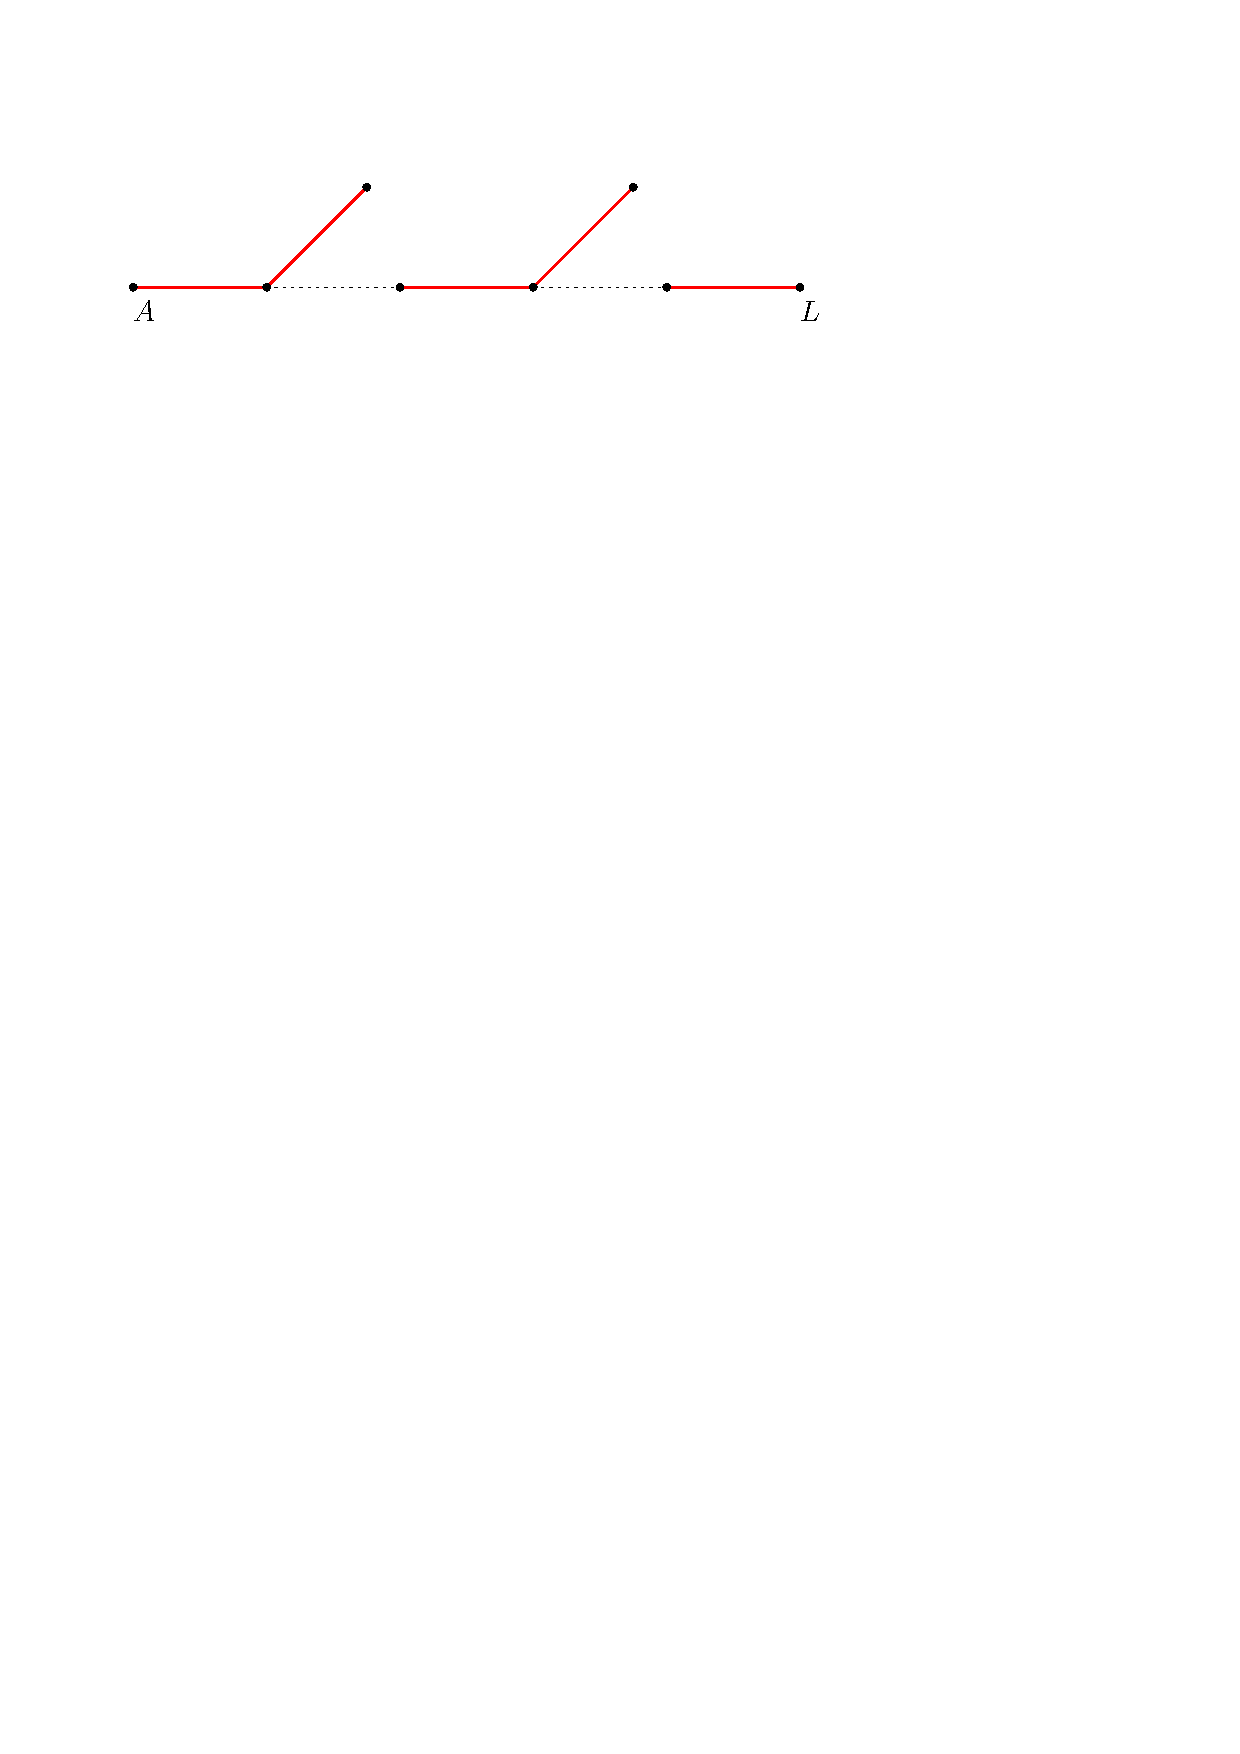
\includegraphics[width=0.8\textwidth]{circuito-em-serie}%
\caption{Forma mnemônica para a conjunção}%
\label{fig:circ-serie}%
\end{figure}

Agora, suponha que eu dissesse assim para Asaph: ``Filhote\ldots vou te dar um
livro ou um carro \textit{Hot Wheels}, em seu aniversário''.
Ou seja, ``$p$ ou $q$''.
Nesse caso, se eu trouxesse, por exemplo, apenas o livro, estaria cumprindo 
minha promessa.
E se eu trouxesse os dois, também (Asaph ficaria ainda mais feliz, não?).
Eu quebraria a promessa se não trouxesse nenhum dos itens!

O que isso nos diz?
Vemos que a \textit{disjunção} só é \F\ (falsa) se ambas proposições são falsas!
Veja a Tabela Verdade da Disjunção (Tabela~\ref{tab:disjuncao}).

\begin{table}[!htbp]%
\centering
\scalebox{0.8}
 {
  \begin{tabular}{ccc}
	  \toprule
    $p$ & $q$ & $p$ ou $q$\\
	  \midrule
    V   &  V  & V\\
	  	V   &  F  & V\\
	  	F   &  V  & V\\
	  	F   &  F  & \F\\
	  \bottomrule
  \end{tabular}
 }
\caption{Tabela Verdade da disjunção}
\label{tab:disjuncao}
\end{table}

Uma forma mnemômica para lembrarmos a disjunção, é pensarmos num circuito 
elétrico em paralelo (Veja a Figura~\ref{fig:circ-para}).
A eletricidade, que sai do ponto $A$, acenderá a luz (ponto $L$) se,
\textit{pelo menos}, uma das chaves estiverem conectadas.
Em outras palavras, só não acenderá a luz se \textit{todas} as chaves estiverem
desconectadas.

\begin{figure}[!h]%
\centering
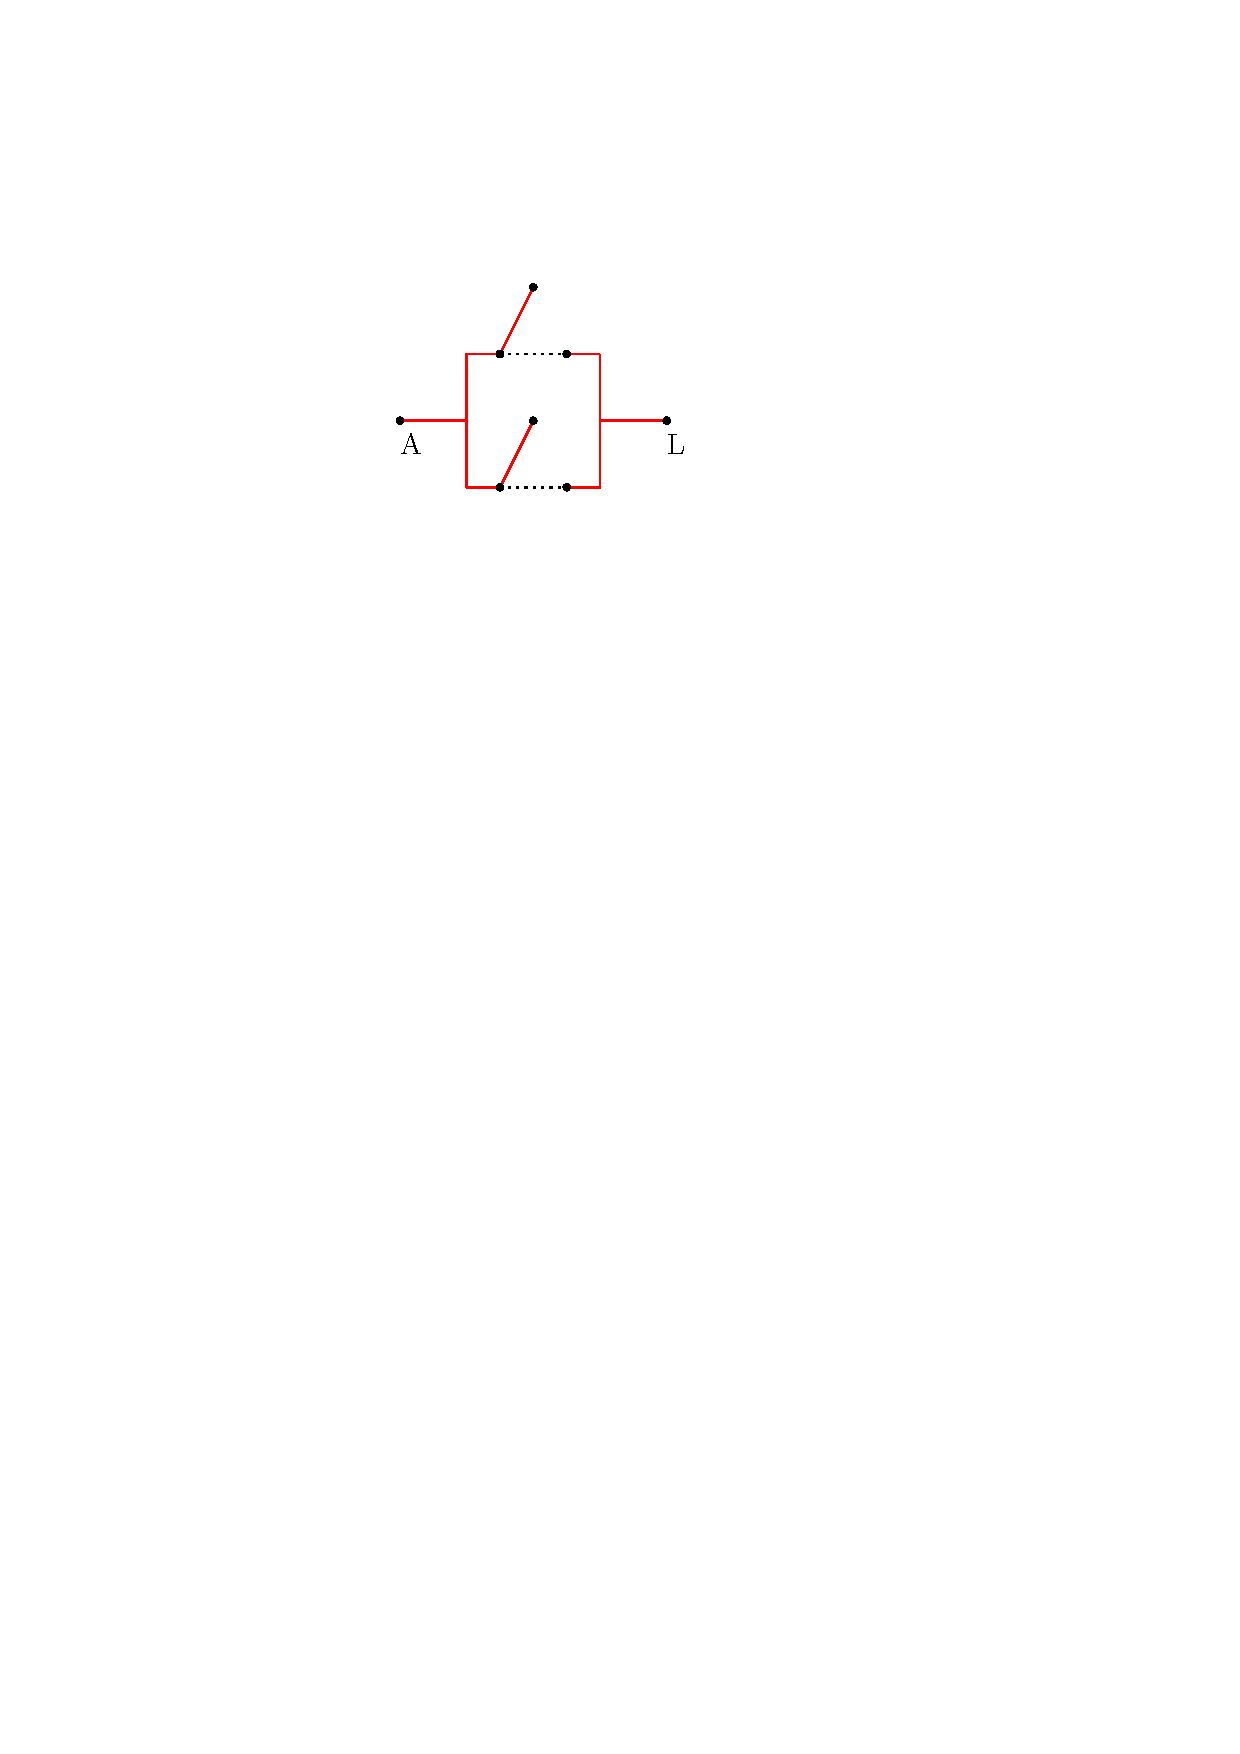
\includegraphics[width=0.4\textwidth]{circuito-em-paralelo}%
\caption{Forma mnemônica para a disjunção}%
\label{fig:circ-para}%
\end{figure}

Poderíamos fazer outras tabelas verdades para os outros conectivos, todavia não
vamos precisar deles para o entendimento matemático do Argumento de Draper.
Entretanto, é conveniente expressarmos a tabela verdade do modificador, ou seja,
a negação de uma proposição $p$. Antes, porém, vamos detonar a operação de
\textit{negação} por ``$\sim$'', ou seja, ao escrevermos ``$\N p$'', estamos
negando a proposição $p$. Veja a Tabela~\ref{tab:negacao}.

\begin{table}[!htbp]%
\centering
\scalebox{0.8}
 {
  \begin{tabular}{cc}
	  \toprule
    $p$ & $\N p$ \\
	  \midrule
    V   &  \F  \\
	  	F   &  \V  \\
	  \bottomrule
  \end{tabular}
 }
\caption{Tabela Verdade da Negação}
\label{tab:negacao}
\end{table}

Agora, podemos combinar algumas coisas simples para podermos definir certos
conceitos usados no Argumento de Draper.

Considere a proposição ``$p$ e $\N p$'', composta pelas proposições $p$ e sua
negação\ldots 
Como seria a tabela verdade para essa proposição composta?

Não é difícil perceber que o resultado só terá valor lógico \F, como na 
Tabela~\ref{tab:contradicao}.
Quando isso acontece, ou seja, quando o \textit{único} valor lógico possível no
resultado é ``\F'', independentemente dos valores lógicos de entrada iniciais,
temos uma \textit{contradição}.

\begin{table}[!h]%
\centering
 \scalebox{0.8}
	{
  \begin{tabular}{ccc}
   \toprule
   $p$ & $\N p$ & $p$ e $\N p$\\
		 \midrule
   V   & F      & \textbf{\textcolor{red}{F}} \\
		 F   & V      & \textbf{\textcolor{red}{F}}\\
   \bottomrule
  \end{tabular}
	}
\caption{Uma contradição}
\label{tab:contradicao}
\end{table}

Caso o \textit{único} valor lógico possível no resultado seja ``\V'', temos uma
\textit{tautologia}.
Veja, por exemplo a Tabela~\ref{tab:tautologia}, que expressa a tabela verdade
da proposição composta ``$p$ ou $\N p$''.

\begin{table}[!h]%
\centering
 \scalebox{0.8}
	{
  \begin{tabular}{ccc}
   \toprule
   $p$ & $\N p$ & $p$ ou $\N p$\\
		 \midrule
   V   & F      & \textbf{\textcolor{red}{V}} \\
		 F   & V      & \textbf{\textcolor{red}{V}}\\
   \bottomrule
  \end{tabular}
	}
\caption{Uma tautologia}
\label{tab:tautologia}
\end{table}

E se o resultado possível não for \textit{somente} \V ou \textit{somente} \F\,?
Ou seja, se houver tanto \V\ como \F\ no resultado final?
Melhor ainda: se o resultado final de uma proposição composta não for nem uma
contradição, nem uma tautologia, então será uma \textit{contingência}.
Volte e reveja a Tabela~\ref{tab:conjuncao} ou  a Tabela~\ref{tab:disjuncao}:
elas expressam proposições compostas que são contingências.

Notem bem o significado de uma ``\textit{não} contingência'': se uma proposição
é não contingente, então será ou uma tautologia, ou uma contradição.
Em outras palavras, o resultado da proposição composta só poderia assumir ou o 
valor lógico \V, ou o valor lógico \F, independentemente dos valores lógicos
assumidos inicialmente pelas proposições simples.
No livro, Plantinga, expressa esse pensamento de ``não contingência'' como:
\textit{necessariamente verdadeiro} ou \textit{necessariamente falso}.  

Apenas para representar visualmente a relação entre essas definições, considere
$A$ o conjunto de todas as proposições compostas que possuem como resultado
\textit{pelo menos} um valor lógico \V. 
Da mesma forma, considere $B$ o conjunto de todas as proposições compostas que
possuem como resultado \textit{pelo menos} um valor lógico \F.
Veja a relação na Figura~\ref{fig:diagrama-contingencia}

\begin{figure}[!h]%
\centering
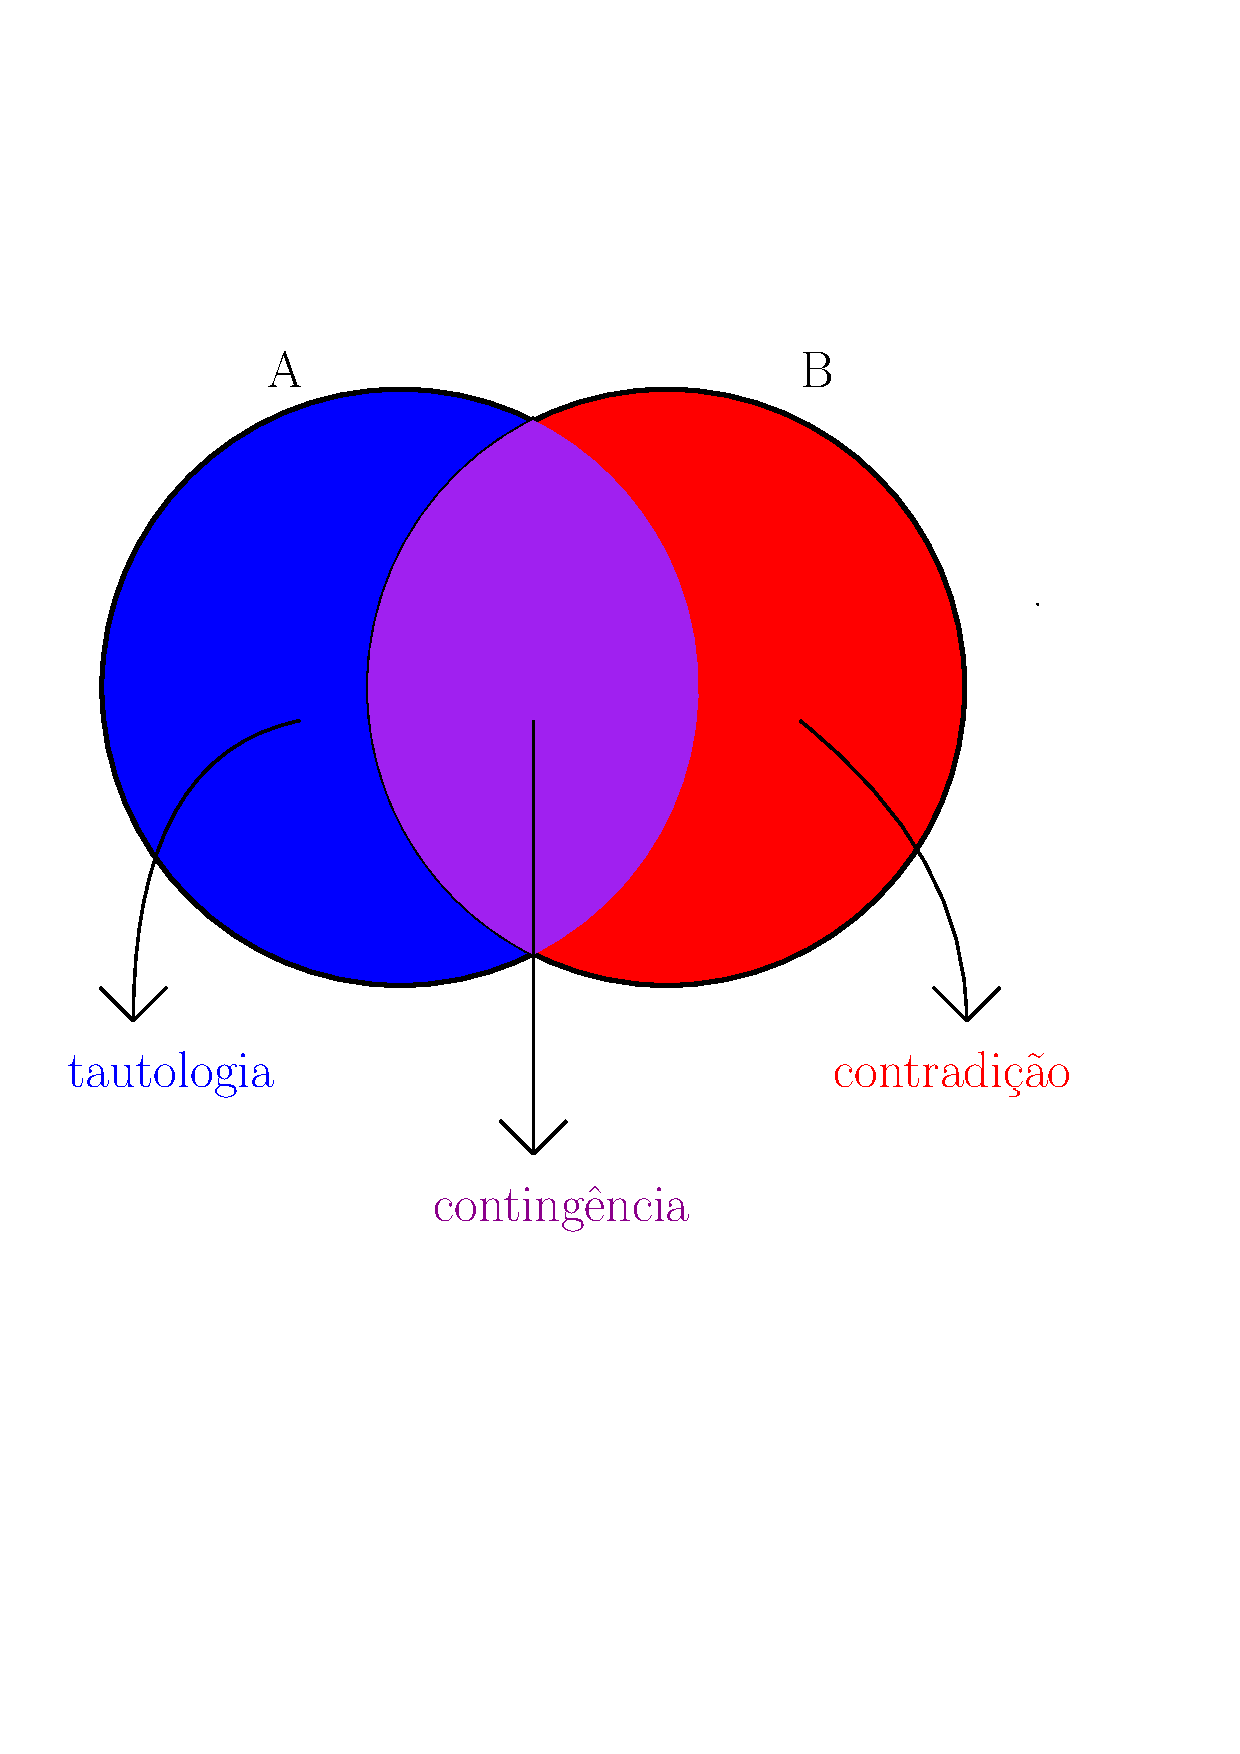
\includegraphics[width=0.6\textwidth]{diagrama-contingencia}%
\caption{Tautologia, Contingência e Contradição}%
\label{fig:diagrama-contingencia}%
\end{figure}
%------------------------------------------------------------------------------

%------------------------------------------------------------------------------
% Probabilidade 
%------------------------------------------------------------------------------
\section{Probabilidade}
Quando o professor Glênon colocou os papeis (os quais confiamos que estivessem
cortados semelhantemente) com as iniciais dos nomes de quatro professores 
(incluindo o seu próprio nome) numa urna improvisada, para sortear 
qual grupo apresentaria primeiro; ele estava realizando um \textit{experimento 
aleatório}.
Ou seja, é \textit{aleatório}, um experimento que, se repetido sob as mesmas 
condições, pode gerar resultados diferentes.

Os quatro grupos foram representados pelas iniciais: $G, Y, H\text{ e } I$.
Se representarmos por $\Omega$, o conjunto de todos os resultados possíveis 
desse experimento feito por Glênon, poderíamos afirmar que:
\[
  \Omega = \left\{\,G, Y, H, I\,\right\}.
\] 
Chamamos $\Omega$ de \textit{espaço amostral}.
Ora, todo subconjunto de $\Omega$ é denominado \textit{evento}.
Mesmo, aqueles impossíveis! 
Por exemplo, se alguém quisesse saber a possibilidade de sair a inicial $L$ do
nome do professor Lucas nesse experimento, falaríamos que tal possibilidade não
está definida no experimento (de forma direta).
Portando, se $E_1$ representasse tal possibilidade, teríamos $E_1 = \varnothing$
(que é o conjunto vazio).

De uma forma geral, se $E$ e $F$ são eventos de um espaço amostral $\Omega$, 
algumas relações entre esses eventos se destacam.
Dentre esses destaques há, por exemplo: $E\cup F$, que representa a ocorrência
de, \textit{pelo menos}, um dos eventos ($E$ ou $F$); e, $E \cap F$, que 
representa a ocorrência \textit{simultânea} desses eventos ($E$ e $F$).
Quando $E$ e $F$ não são simultâneos, ou seja, quando $E\cap F = \varnothing$,
dizemos que os eventos são \textit{mutualmente excludentes}.

Agora, ainda em nosso experimento do sorteio das apresentações do Contraponto,
suponha que alguém queira saber a chance de ser sorteada a inicial de algum 
professor que aparenta ter mais do que 50 anos.
Bom, se $E_2$ é esse evento, temos apenas três possibilidade (como é evidente): 
\[
  E_2 = \left\{\, G, Y, H \,\right\} 
\]
Portanto, o que chamamos de \textit{chance} é a razão do número de 
\textit{casos favoráveis} pelo número de \textit{casos possíveis}.
No exemplo, temos 3 casos favoráveis dentre 4 possíveis; logo, a chance de ser
sorteado algum professor que aparenta ter mais do que 50 anos é de $3/4$ (ou
0.75, ou 75\%).

Assim, intuitivamente:

\[
  \text{Probabilidade } = 
		\frac
		 {
			 \text{ nº de casos favoráveis }
			}
			{
			 \text{ nº de casos possíveis}
			}
\]

Vamos denotar\footnote{No livro, usa-se a notação $P$ ou invés de $\Pr$. 
Prefiro a segunda, pois já passei por situações constrangedoras ao usar a 
notação $P(A)$ (``pê de A'') --- fale várias vezes em voz alta, para você ver!} 
a \textit{probabilidade} de ocorrência de um evento $E$ por $\Pr{(E)}$. 

Agora, por que afirmei ``intuitivamente'' quando tentei formalizar o conceito de
probabilidade?
Ora, estamos supondo que a chance de sair qualquer inicial é a mesma, ou seja, 
\[
  \Pr{(G)} = \Pr{(Y)} = \Pr{(H)} = \Pr{(I)} .
\]
Mas, e se professor Glênon, proposital e disfarçadamente, cortou seu papel maior
do que os dos outros professores para poder aumentar as suas chances de ser o 
primeiro a apresentar e, assim, não correr o risco de apresentar os próximos 
capítulos (os quais aumentam em complexidade nos assuntos)?

Vamos supor que a forma que ele cortou o papel, fez com que a chance de 
sair a inicial $G$ fosse de $0.5$; a inicial, $Y$, do amigo de longas datas,
Yuji, fosse de $0.3$ e a dos outros dois professores envolvidos no sorteio 
fosses iguais a $0.1$, cada.
Dessa forma, a ideia de \textit{probabilidade} pode ser relacionada a uma 
função, que associa um evento a um número real (no intervalo $[0, 1]$) que, de
alguma forma, expresse a nossa \text{fé} (ou medida de confiança) na ocorrência
desse evento.

Esse é o conceito adotado atualmente: a forma axiomática de probabilidade.
Vamos formalizar\newline (usando uma linguagem básica) isso na Definição\ref{def:prob}.

\begin{definicao}\label{def:prob}
Uma \textit{probabilidade} é uma função 
\[
  \begin{array}{rcc}
   \Pr \colon \Omega & \longrightarrow & \mathbb{R}\\
		 E                 & \mapsto     & \Pr{(E)}
		\end{array}
\]
que associa cada evento, $E\in\Omega$, um número real, $\Pr{(E)}$, tal que:
\begin{enumerate}[(1)]
	\item $ 0 \leq \Pr{(E)} \leq 1 $;
	\item $ \Pr{(\Omega)} = 1 $;
	\item Se os eventos $ E $ e $ F $ são \textit{mutualmente excludentes}, então
	$ \Pr{(A \cup B)} = \Pr{(A)} + \Pr{(B)}$ .
\end{enumerate}
\end{definicao}

O item~(2)\footnote{É possível mostrar, com esses axiomas dados, que 
$\Pr{(\varnothing)} = 0$. Tente demonstrar!} pode ocorrer, em nosso exemplo, se 
quiséssemos saber, por exemplo, a probabilidade de sair a inicial de algum 
professor da UFRB. 
Ora, todos os professores envolvidos são professores da UFRB, portanto, a chance
disso ocorrer é \textit{certa}.
Em outras palavras, analisamos a ocorrência do evento 
$ E = \left\{\,G, Y, H, I\,\right\} $ no espaço amostral com os mesmos elementos,
a saber, $ \Omega = \left\{\,G, Y, H, I\,\right\} $.
Assim, temos 4 casos favoráveis, num total de 4 possíveis, o que dá a 
probabilidade de $1$.

Vejam que não há contradição entre uma definição e outra.
Na Definição~\ref{def:prob} está contida o caso em que os eventos são 
\textit{equiprováveis}.

Até aqui, falamos sobre a probabilidade calculada \textit{antes} do resultado
do experimento.
Vou fazer igual ao Plantinga e usar o Latim (hehehe): esse tipo de probabilidade
é dita \textit{a priori}.
Mas, a probabilidade envolvida no Argumento de Draper, é do tipo 
\textit{a posteriori}, ou seja, calculamos a probabilidade depois de alguma
informação extra, advinda do experimento.
Precisamos falar sobre Probabilidade Condicional e, por simplicidade, trataremos
dos conjuntos finitos (ou os infinitos enumeráveis, mas se você nunca ouviu
falar nisso, não vai influenciar no entendimento).
%------------------------------------------------------------------------------
% Prob.--- Condicional
%------------------------------------------------------------------------------
 \subsection{Probabilidade Condicional}
  Vamos voltar ao nosso exemplo do sorteio das apresentações do contraponto.
		Vamos confiar em nosso colega e professor Glênon e supormos o experimento
		aleatório e equiprovável.
		
		Então, se eu pergunto: ``qual a probabilidade de sair a inicial do nome do 
		professor Hugo nesse sorteio?''
		Certamente você me responderia: $ \Pr{(H)} = 1/4 $.
		
		Agora, vamos imaginar a situação, hipotética, de Glênon (após um leve sorriso
		maroto) ter falado, assim que olhou para o papel sorteado: ``Olha\ldots não
		foi a minha inicial que saiu aqui no papel!''.
		
		E agora?
		Se eu perguntasse: ``qual a probabilidade de ter saído a inicial do professor
		Hugo nesse sorteio?''
		Se você pudesse calcular a probabilidade, agora, você mudaria o resultado?
	
	 Perceba que, agora, como temos essa informação extra de que não foi a inicial
		do professor Glênon que saiu, o nosso espaço amostral foi reduzido!
		Sim!
		Ficamos, apenas, com $\Omega^\prime = \left\{\, H, Y, I\,\right\}$.
		Logo, temos 1 caso favorável (sair $H$) num total de 3 casos possíveis, o que
		resulta na probabilidade $1/3$.
		
		Em outras palavras, eu perguntei: ``qual a probabilidade de ter saído a 
		inicial $H$ \textit{dado que} não saiu a inicial $G$''?
		
		Para denotarmos a probabilidade de $F$ \textit{dado que} ocorreu $E$, usamos
		uma barra vertical entre os eventos, ficando assim: $ \Pr{(F \mid E)} $.
		
		Tudo bem, mas como podemos calcular, efetivamente, essa probabilidade?
		Para isso, observe a Figura~\ref{fig:diagrama-condicional}.
		
		\begin{figure}[!h]%
		 \centering
		 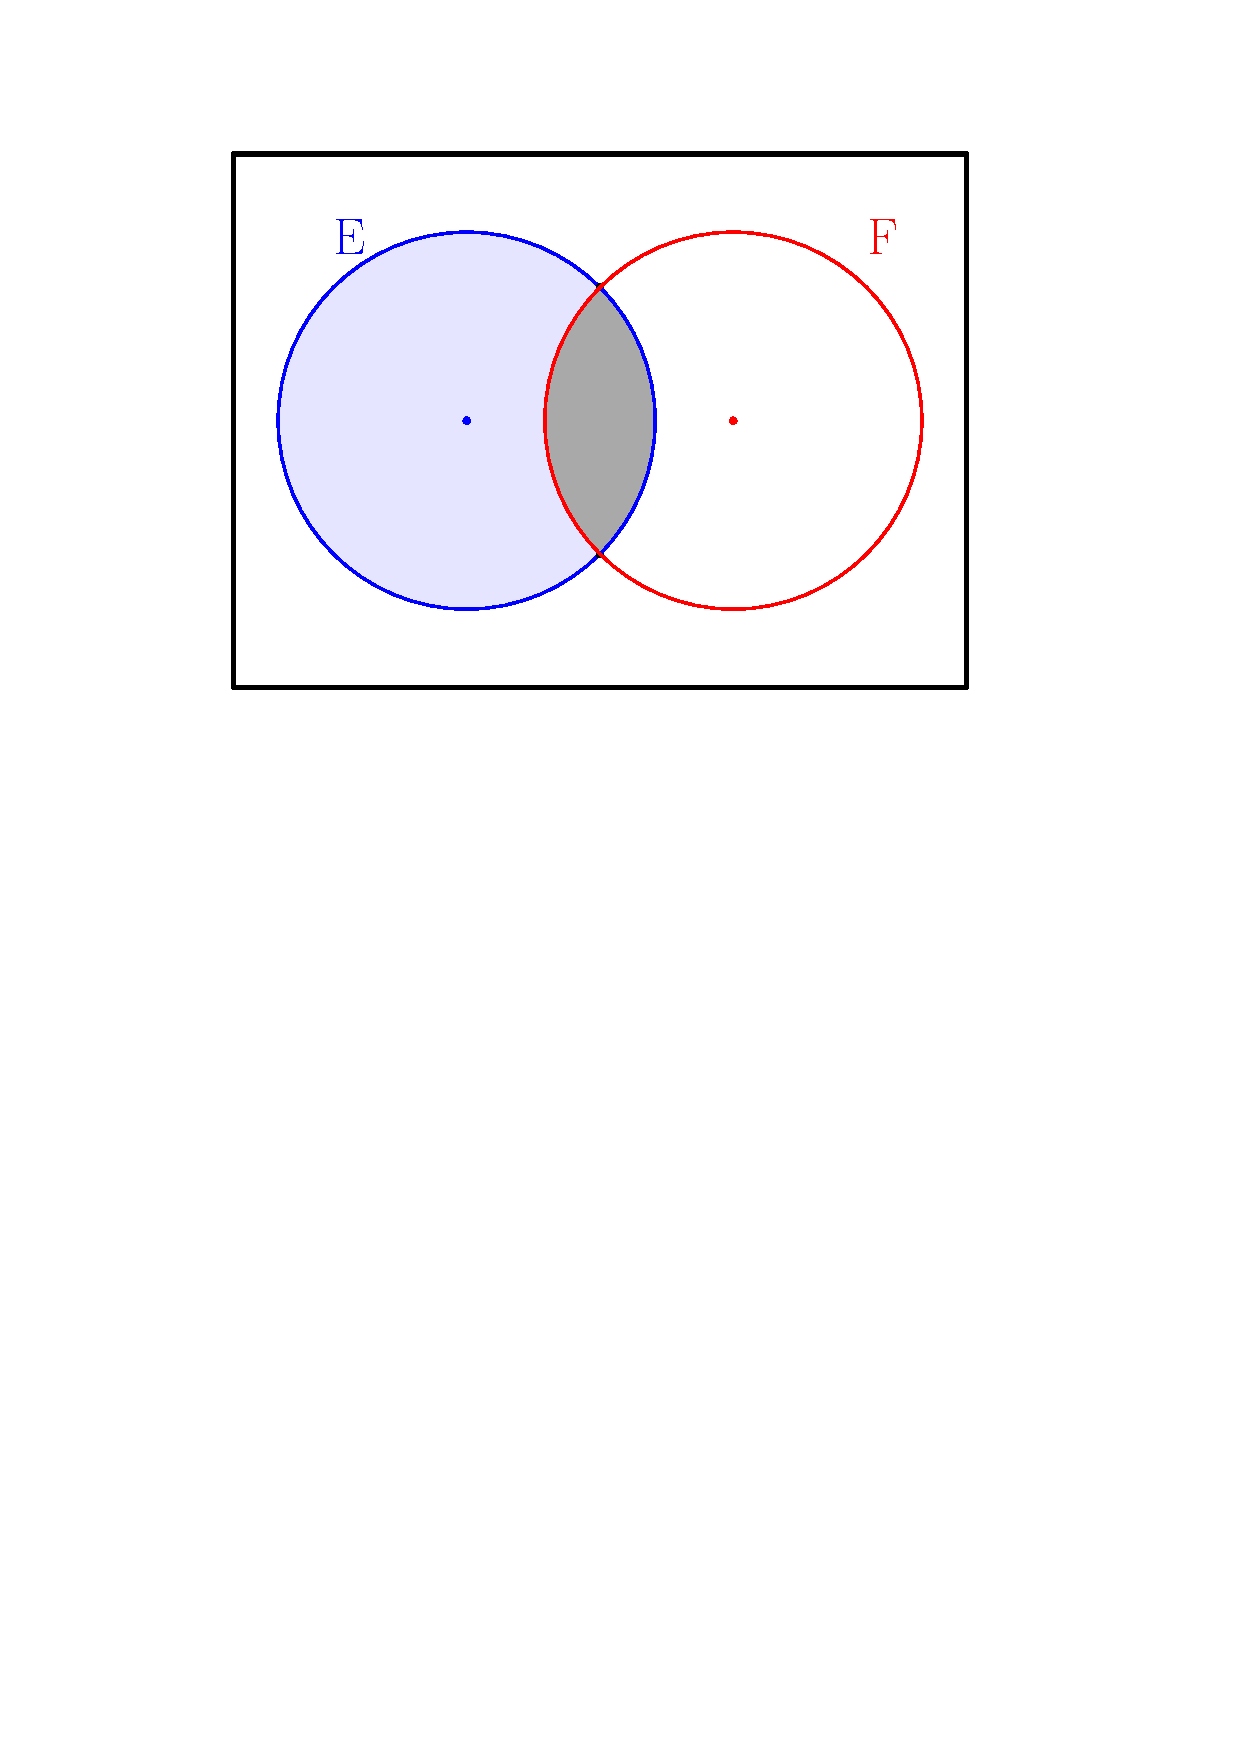
\includegraphics[width=0.5\textwidth]{diagrama-condicional}%
		 \caption{Probabilidade Condicional $\Pr{(F \mid E)}$}%
		 \label{fig:diagrama-condicional}%
		\end{figure}
		
		Como é sabido, ocorreu o evento $ E $.
		Logo, nosso espaço amostral é reduzido ao evento $E$.
		Então, para que ocorra o evento $ F $, dado que ocorreu o evento $E$, aquele
		deve acontecer na interseção dos	eventos, ou seja, em $ E \cap F $. 
		
		Lembre-se de nosso exemplo: ``qual a probabilidade de sair $H$, dado que não
		saiu $G$?''. 
		O nosso espaço amostral inicial era $\Omega = \left\{\, G, Y, H, I\,\right\}$,
		mas, quando soubemos da informação de que não saiu $G$, o espaço amostral
		foi reduzido para
		\[
		 \N G = \left\{\, Y, H, I\,\right\}.
		\]
		Assim, a interseção de $H$ com $\N G$ é dada por:
  \[ 
			H \cap (\N G) = \left\{\, H \,\right\} \cap \left\{\, Y, H, I\,\right\}
				             = \{\, H \,\}
		\]
		Logo, se denotarmos o número de elementos de\\ $ H \cap (\N G)$ por
		$\#\big( H \cap (\N G) \big)$, temos:
		\[
		 \#\big( H \cap (\N G) \big) = 1
		\] 
		Da mesma forma, o número de elementos de $\N G$ é:
		\[
		 \# (\N G) = 3,
		\]
		assim:
		\begin{align}
		 \Pr{\left( H \mid \N G\right)} 
			&= 
			\frac{\#\big( H \cap (\N G) \big)}{\# (\N G)}\label{eq:prob-num}\\
			&= 
			\frac{1}{3} \nonumber
		\end{align}
		Agora, como queremos estabelecer uma maneira de calcular efetivamente a 
		probabilidade condicional, podemos dividir, numerador e denominador, a 
		equação~\ref{eq:prob-num} pelo número de elementos do espaço amostral, a 
		saber, $ \# (\Omega) $. 
		Assim:
		\begin{align*}
		 \Pr{\left( H \mid \N G\right)} 
			&= 
			\frac{\#\big( H \cap (\N G) \big)}{\# (\N G)}\label{eq:prob-num}\\
			&=
			\frac
			{
			 \#\big( H \cap (\N G) \big) / \# (\Omega)
			}
			{
			 \# (\N G) / \# (\Omega)
			}
		\end{align*}
		
		Portanto,
		\[
			\Pr{(H \mid \N G)} = \frac{\Pr{\big(H \cap (\N G)\big)}}{\Pr{(\N G)}}
		\]
	 Isso nos permite definir a probabilidade condicional da seguinte forma:
		
		\begin{definicao}[Probabilidade Condicional]\label{eq:prob-condicional}
		 Dados dois eventos $ E $ e $ F $, com $ \Pr{(E)} \neq 0 $, definimos a 
			\textit{probabilidade condicional} de $ F $, dado que ocorreu $E$, por:
				\[
				 \Pr{(F \mid E)} = \frac{\Pr{\left(F \cap E\right)}}{\Pr{(E)}}.
				\]
		\end{definicao}
		
		Também é importante usarmos essa expressão escrita assim\footnote{obviamente,
		também podemos fazer (é só mudar a ordem): $\Pr{(E \cap F)} = \Pr{(F)}
		\Pr{(E \mid F)}$.}:
		\begin{equation}\label{eq:prop-inter}
		 \Pr{\left(F \cap E\right)} = \Pr{(E)}\Pr{(F \mid E)}
		\end{equation}
	
		Com o exposto até aqui, podemos entender o desenrolar do Argumento de Draper.
		Obviamente, a linguagem que usaremos é interpretativa e básica, não a 
		linguagem axiomática da \textit{probabilidade epistêmica}.
%------------------------------------------------------------------------------

%------------------------------------------------------------------------------
% Argumento de Draper
%------------------------------------------------------------------------------
\section{Argumento de Draper}
	\subsection{Um Alerta!}
	 Apenas ratificando o que escrevi acima: usaremos uma linguagem 
		\textit{interpretativa} e \textit{básica}.
		
		Algumas vezes, pelo bem da simplicidade, usamos de ferramentas ou notações
		que não estão	corretas \textit{no sentido formal da Matemática}, mas que 
		ajudam na simplificação de	simbologias, bem como no entendimento geral da 
		questão.
		
		Por exemplo, se no experimento de lançar uma moeda, o meu espaço amostral for
		$ \Omega = \{\,\text{cara}, \text{coroa}\,\} $, dizemos que a probabilidade de 
		sair ``cara'' (suponha $ \Omega $ equiprovável) é ``$\Pr{(\text{cara})}$'', 
		mas, formalmente seria: ``$\Pr{(\{\text{cara}\})}$'', visto que estamos 
		calculando a probabilidade de um conjunto.
		
		Ora, tudo que vimos de teoria básica  de probabilidade até aqui, trata-se do
		cálculo dessas probabilidades em conjuntos com \textit{certas propriedades}.
		É que não falei delas logo de cara para não ficar chato! 
		Mas, a verdade é que precisamos de uma \textit{álgebra Booleana}, 
		$\mathcal{B}$, cujos elementos são subconjuntos de um conjunto 
		finito\footnote{podemos usar conjuntos infinitos, mas devem ser enumeráveis ---
		mas, isso é outra história} dado: $ \Omega $; e, de uma \textit{função de
		probabilidade}, $\Pr$, cujo domínio é $\mathcal{B}$ e que satisfaça as 
		propriedades que já listamos na Definição~\ref{def:prob}. 
		
		E qual o porquê de falar isso tudo?
		Porque no livro, subentende-se que as ``probabilidades'' ali envolvidas são
		relacionadas às proposições, ou à lógica epistêmica.
		Então, estaríamos falando de ``probabilidade epistêmica'', por assim dizer.
		
		Quais as operações nesse ``tipo'' de probabilidade?
		Existe diferenças entre a ``probabilidade dos conjuntos'' e a ``probabilidade
		epistêmica''?
		São questões interessantes e o livro não fala sobre isso!
		
		Na lógica epistêmica (coisa maluca que foge ao escopo desse texto e às minhas
		capacidades --- pois, sigo, de forma literalista, o Sl 131.1 ), eles 
		axiomatizam	a probabilidade condicional.
		Usam a \href{https://plato.stanford.edu/entries/reasoning-defeasible/suppl4.html#:~:text=A\%20Popper\%20function\%20is\%20a,D\%20\%E2\%88\%A3\%20E\%20\%5D\%20\%E2\%89\%A0\%201\%20.}{Função de Popper},
		a saber, dada uma linguagem $L$, a função 
		$ P \colon L \times L \to \mathbb{R} $ relaciona os pares de proposições aos 
		números reais, da seguinte forma\footnote{entenda ``\&'' como o conectivo ''e''}:
			
		\begin{enumerate}[(i)]
			\item Para todo $A, B$, existe $C$ e $D$, tal que\\ $P(A\mid D) \neq P(C\mid D)$;
			\item Se $P(A\mid C)=P(B\mid C)$, para todo $C$, então 
			 $P(D\mid A)=P(D\mid B)$, para todo $D$;
			\item $P(A\mid A) = P(B\mid B)$;
			\item $P\big((A \& B)\mid C\big) \leq P(A\mid C)$;
			\item \textcolor{blue}{$P\big((A \& B) \mid C\big) = P(B\mid C)\cdot P\big(A\mid (B \& C)\big)$};
			\item $P(A\mid B) + P(\N A\mid B) = P(B\mid B)$, exceto quando 
			 $P(B\mid B) = P(C\mid B)$, para todo $C$.
		\end{enumerate}
		
		Pois é \ldots a linguagem é um tanto árida, não?
		Mas, o que vai nos interessar é o item~(v):	Draper o usa diretamente.
		
		Em outras palavras, eu não precisaria escrever todos esse texto falando de 
		lógica, probabilidade e probabilidade condicional.
		Bastaria escrever esses axiomas e falar que o Draper usou o 5º deles\footnote{
		também conhecido como ``regra do produto'', ou ``axioma da multiplicação''.}.
		Mas, não teria graça, não?
		
		A ideia do presente texto é tentar usar uma linguagem mais ``acessível'' para
		mostrar	a plausabilidade da afirmação que Draper usa.
		Não achei direta, nem trivial à primeira vista.
		
		Agora, eu estou supondo que essa linguagem é semelhante à axiomatização de
		Popper.
		Pelo menos é isso que o Plantinga deixa claro nos cálculos que ele faz.
		Então, lembre-se\footnote{hehehehe}:
		
		\begin{center}
		 \Ovalbox
		 {
		  \textbf{\textcolor{red}{Se o Plantinga estiver errado, também estarei!}}
		 }
		\end{center}
		
%------------------------------------------------------------------------------	
	\subsection{Considerações sobre o Argumento}
	
	 Para compreendermos (matematicamente) o argumento, vamos relembrar as notações
		usadas: 
		
		\begin{center}
		 \begin{tabular}{rl}
		  $E$: & Evolução (\textit{Evolution});\\
			 $T$: & Teísmo (\textit{Theism});\\
			 $N$: & Naturalismo (\textit{Naturalism});\\
			 $S$: & Criação Especial (\textit{Special Creation}).
		 \end{tabular}
		\end{center}
		
		Aqui, precisamos levantar algumas questões referentes ao que está exposto no
		livro sobre ``Evolução'' e ``Criação Especial''.
		De acordo com Plantinga, Draper diz sobre:
		
		\begin{itemize}
		 \item \textbf{Evolução}: \textit{é a proposição de que todas as formas de 
			vida terrestre existentes na época atual surgiram por meio da evolução}.
			\item \textbf{Criação Especial}: \textit{alguns seres vivos relativamente 
			complexos não descendem de organismos unicelulares relativamente simples, 
			mas foram criados independentemente por uma pessoa sobrenatural}.
		\end{itemize}
		
		É notório que a \textit{negação} da ideia de ``Criação Especial'' ($ \N S $)
		contém a ideia da ``Evolução''.
		Em outras palavras $E \subset (\N S)$.
		Portando, Draper argumenta que:
		
		\begin{equation}\label{eq:argumento-draper}
		 \Pr{(E \mid N)} \gg \Pr{(E \mid T)}
		\end{equation}
		
		Ou seja, a ``Evolução, dado o Naturalismo'', é muito mais provável do que a 
		``Evolução'', dado o Teísmo''.
		E, para mostrar essa argumentação, ele usa a seguinte desigualdade:	
		
		\scriptsize
		\begin{equation} \label{eq:draper-logica}
		 \textcolor{red}{\Pr{(\N S \mid N)}} \cdot \Pr{\big(E \mid (\N S \& N)\big)}
		 \gg
		 \textcolor{red}{\Pr{(\N S \mid T)}} \cdot \Pr{\big(E \mid (\N S \& T)\big)}
		\end{equation}
		\normalsize
		
		Foi essa desigualdade que não foi tão direta para mim, numa primeira leitura.
		E, com o que desenvolvemos até aqui, podemos verificar a validade da mesma.
		Vejamos\ldots
		
		Estamos supondo $ E \subset (\N S) $, ou seja, a ideia de ``Evolução'' está
		contida na negação de uma criação especial das espécies; portanto, 
		$ E \cap (\N S) = E $, ou melhor, $ E \& (\N S) = E $.
		Mas, usaremos a primeira notação para os cálculos.
		
		Assim, usando a Definição~\ref{eq:prob-condicional}, bem como seus 
		desdobramentos (Equação~\ref{eq:prop-inter}):
		
		\footnotesize
		\begin{align*}
		 \Pr{\big(E \mid N\big)} &= \Pr{\big((E \cap \N S) \mid N \big)}\\
			&= \frac{\Pr{\big(E \cap (\N S) \cap N}\big)}{\Pr{(N)}}\\
			&= \frac{\textcolor{blue}{\Pr{\Big(E \cap (\N S \cap N)}\Big)}}{\Pr{(N)}} 
		\end{align*}
		\normalsize
		
		Agora, usando a Equação~\ref{eq:prop-inter}, podemos fazer:
		\footnotesize
		\[
		 \textcolor{blue}{\Pr{\Big(E \cap (\N S \cap N)}\Big)} = \Pr{(\N S \cap N)}\cdot \Pr{\Big(E \mid (\N S \cap N)\Big)}
		\]
		\normalsize
		Assim,
		\footnotesize
		\begin{align*}
		 \Pr{(E \mid N)} &= \frac{\textcolor{blue}{\Pr{(\N S \cap N)}} \cdot \textcolor{blue}{\Pr{\Big(E \mid (\N S \cap N)\Big)}}}{\Pr{(N)}}\\
			&= \frac{\cancel{\textcolor{red}{\Pr{(N)}}} \cdot \textcolor{red}{\Pr{(\N S \mid N)}}
				\cdot
				\textcolor{blue}{\Pr{\Big(E \mid (\N S \cap N)\Big)}}}{\cancel{\Pr{(N)}}}\\
			&= \Pr{(\N S \mid N)} \cdot \Pr{\Big(E \mid (\N S \cap N)\Big)}
		\end{align*}
		\normalsize
		
		Portanto, usando a simbologia do livro:
		\footnotesize
		\begin{equation}\label{eq:draper-a}
		 \Pr{(E \mid N)} = \Pr{(\N S \mid N)} \cdot \Pr{\Big(E \mid (\N S \& N)\Big)}
		\end{equation}
		\normalsize
		
		De forma análoga,
		\footnotesize
		\begin{equation}\label{eq:draper-b}
		 \Pr{(E \mid T)} = \Pr{(\N S \mid T)} \cdot \Pr{\Big(E \mid (\N S \& T)\Big)}
		\end{equation}
		\normalsize
		
		Das Equações~\eqref{eq:draper-a} e \eqref{eq:draper-b}, podemos enxergar a
		equivalência entre as Equações~\eqref{eq:argumento-draper} e 
		\eqref{eq:draper-logica}.
		
		Observe que chegaríamos a mesma conclusão se usássemos o item~(v), da 
		axiomatização de Popper, nas proposições\footnote{ou nas proposições:
		``$E \& (\N S)$'' e ``$T$''} ``$E \& (\N S$)'' e ``$N$''.
%------------------------------------------------------------------------------

%------------------------------------------------------------------------------
% Argumento de Draper --- Diagramas
%------------------------------------------------------------------------------
 \subsubsection{Visualizando a Desigualdade}
	 Uma possível visualização da equivalência entre as 
		Equações~\eqref{eq:draper-a} e \eqref{eq:draper-b}, encontra-se na 
		Figura~\ref{fig:draper-visu}.
		
	 \begin{figure}[!htbp]%
		\centering
		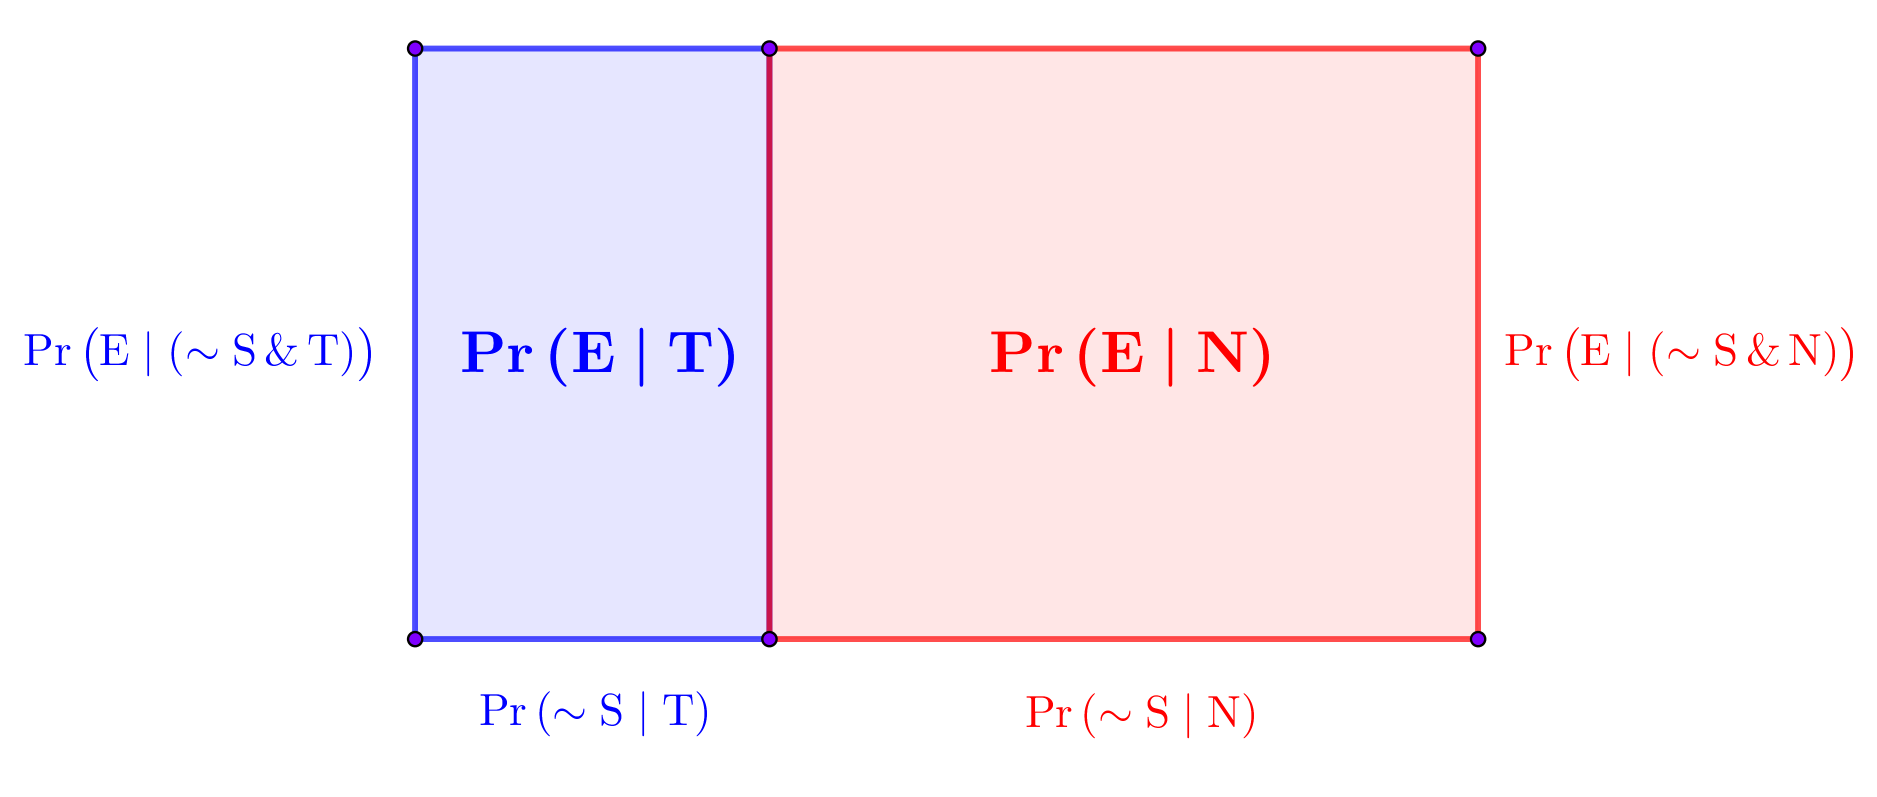
\includegraphics[width=\textwidth]{diagrama-visu}%
		\caption{Uma possível representação}%
		\label{fig:draper-visu}%
		\end{figure}
		
		Para interpretarmos tal representação visual, considere o que Draper, segundo
		Plantiga, afirma:
		
		\vspace{0.3cm}
		\footnotesize
		\noindent``$\Pr{\big(E\mid (\N S \,\&\, N)\big)}$
		é \textit{tão grande quanto}
		$\Pr{\big(E\mid (\N S \,\&\, T)\big)}$''.
		\normalsize\\
		
		Então, a probabilidade $\Pr{(E\mid N)}$ é a área do retângulo de lado
		$\Pr{(\N S \mid N)}$ e altura \[\Pr{\big(E\mid (\N S \,\&\, N)\big)},\] bem como
		$\Pr{(E\mid T)}$ é a área do retângulo de lado
		$\Pr{(\N S \mid T)}$ e altura \[\Pr{\big(E\mid (\N S \,\&\, T\big)}.\]
		
		Portanto, se você mantém fixa as alturas de dois retângulos, para mostrar que 
		a área de um é maior do que a área de outro, basta mostrar que o lado de um
		é maior do que o lado do outro.
		
		E foi isso que o Draper tentou fazer: manteve \textit{arbitrariamente} as
		proporções $\Pr{\big(E\mid (\N S \,\&\, N)\big)}$ e 
		$\Pr{\big(E\mid (\N S \,\&\, T)\big)}$ fixas e argumentou que\\
		$\Pr{(\N S \mid N)}$ é \textit{pelo menos duas vezes maior do que} 
		$\Pr{(\N S \mid T)}$.
		
		Em outras palavras, Draper, construiu um arcabouço de argumentações baseado
		em \textit{pressuposições convenientes}.
		Aí fica fácil, né?
		
		\subsection{Ser ou não ser Contingente}
		Antes de Plantinga contra-argumentar o que Draper afirmou da equivalência 
		entre as Equações~\eqref{eq:draper-a} e \eqref{eq:draper-b}, ele fez uma 
		afirmação contundente:
		
		\begin{quote}
		 ``\ldots a probabilidade de uma proposição contingente, dada uma falsidade 
			necessária, é 1.''
		\end{quote}
		
		Confesso que, matematicamente, usando as teorias básicas expostas, não 
		consegui verificar a validade dessa afirmação.
		Provavelmente o Plantinga está usando algum sistema axiomático onde essa 
		afirmação é evidente.
		Mas, no geral, é difícil compreender.
		
		Por exemplo, 
		
		\begin{tabular}{rl}
		 $A$: & ``A Evolução é verdadeira.''\\
			$B$: & ``$2 + 2 = 7.$''
		\end{tabular}
		
		$A$ é uma proposição contingente (pode ser ou não verdadeira) e $B$ é uma
		contradição, ou seja, necessariamente falsa.
		Então, $ \Pr{(A \mid B)} = 1 $?
		Por quê?
		Se pensarmos em termos da Definição~\ref{eq:prob-condicional}, note que:
		\[
		 \Pr{(A \mid B)} = \frac{\Pr{(A \,\&\, B)}}{\Pr{(B)}}
		\]
		Como o valor lógico de ``$A\,\&\, B$'' é \F; e, o valor lógico de $B$ é \F,
		então, de alguma maneira, teria sendido a expressão:
		\begin{align*}
		 \Pr{(A \mid B)} &= \frac{\Pr{(\F)}}{\Pr{(\F)}}\\
			&= 1.
		\end{align*}
		
		Mas, eu não soube precisar tal afirmação.
		Além disso, as passagens matemáticas não estão precisas na especulação acima.
		
		De qualquer forma, \textit{supondo a veracidade dessa afirmação de Plantinga},
		este argumenta que a Equação~\ref{eq:draper-a} não implica, necessariamente,
		que o Naturalismo é mais provável do que o Teísmo, ou seja, que 
		$\Pr{(N)} > \Pr{(T)}$.
		Ao contrário, se $T$ for não contingente, a expressão resulta na veracidade
		do Teísmo.
		
		Com efeito, se $T$ é não contingente, ou ele é uma tautologia, ou ele é uma
		contradição. 
		Se $T$ é uma tautologia, não há mais nada que demonstrar, visto que o Teísmo
		seria verdadeiro.
		Mas, se $T$ for uma contradição, a desigualdade da 
		Equação~\ref{eq:argumento-draper},	ou seja, 
		$ \Pr{(E \mid N)} \gg \Pr{(E \mid T)} $, não se sustentaria, visto que 
		teríamos $\Pr{(E\mid T)} = 1$, logo $\Pr{(E \mid N )}$ deveria ser maior do
		que 1, o que é um absurdo (lembre-se que $0\leq\Pr{(A)}\leq 1$, para todo 
		$A$).
		
\section{Conclusão}
É isso pessoal!
Esse foi um pequeno texto informal para lançar um pouco mais de luz ao 
entendimento da contra-argumentação de Plantinga ao que Draper propõe.

É notório que, como diria Glênon, tudo depende dos pressupostos adotados!
Mesmo a Evolução, não implica necessariamente o Naturalismo.
Algumas outras hipóteses convenientes (e questionáveis) sempre são postas na
argumentação, o que enfraquece o argumento como um todo.

Então, mesmo que em algum momento a argumentação do Plantinga não esteja tão
clara para mim, as conclusões do Draper são forçadas e dependentes de um 
conjunto de considerações construídas arbitrariamente para favorecer seu 
argumento.

Espero que o texto tenha ajudado! 
%------------------------------------------------------------------------------

\end{document}
%==============================================================================
